\documentclass [a4paper] {article}

\usepackage[dvipsnames]{xcolor}

\usepackage{fancyvrb}

\RecustomVerbatimCommand{\VerbatimInput}{VerbatimInput}
{fontsize=\footnotesize,frame=lines,framesep=2em,rulecolor=\color{Gray},commandchars=\|\(\),commentchar=*}

\title{R-PL1}
\author{Gabriel L\'opez, Sergio Sanz, \'Alvaro Zamorano}

\usepackage{Sweave}
\begin{document}

\maketitle

A lo largo de la pr\'actica usaremos una funci\'on creada por nosostros para almacenar los resultados obtenidos en un .txt y posteriormente
mostrarlos de forma correcta, por ello es necesario ejecutar:
\begin{Schunk}
\begin{Sinput}
> source("toTXT.R")
> toTxt
\end{Sinput}
\begin{Soutput}
function(save,name,r) {
    write.table(save, paste("./tmp/",name,sep=""), sep="\t", row.names=r) 
}
\end{Soutput}
\end{Schunk}

\graphicspath{ {./tmp/} }

En esta parte de la pr\'actica trabajaremos con el fichero
\texttt{satelites.txt}.\\

\bigskip
En primer lugar hay que leer este fichero, para ello usamos
la funci\'on:
\begin{Schunk}
\begin{Sinput}
> satelites<-read.table("satelites.txt")
\end{Sinput}
\end{Schunk}

\bigskip
Para trabajar con la variable radio, y hacer este trabajo m\'as
c\'omodo, la cargamos en una variable:
\begin{Schunk}
\begin{Sinput}
> Radio<-satelites$Radio
\end{Sinput}
\end{Schunk}

\bigskip
En el primer an\'alisis de los datos se cuantifica la \textbf{frecuencia}
de aparici\'on de los mismos. 

\begin{enumerate}
\item
\textit{Frecuencia absoluta: }
\begin{Schunk}
\begin{Sinput}
> frabsradio<-table(Radio)
> toTxt(frabsradio,"frabsradio.txt",F)
\end{Sinput}
\end{Schunk}
\VerbatimInput{./tmp/frabsradio.txt}

\item
\textit{Frecuencia absoluta acumulada: }
\begin{Schunk}
\begin{Sinput}
> frabsacumradio<-cumsum(table(Radio))
> toTxt(frabsacumradio,"frabsacumradio.txt",T)
\end{Sinput}
\end{Schunk}
\VerbatimInput{./tmp/frabsacumradio.txt}

\item
\textit{Frecuencia relativa: }En este caso es necesario crear una funci\'on
para poder calcular este valor. La funci\'on es:
\begin{Schunk}
\begin{Sinput}
> frecrel<-function(Radio){table(Radio)/length(Radio)}
> frer<-frecrel(Radio)
> toTxt(frer,"frer.txt",F)
\end{Sinput}
\end{Schunk}
\VerbatimInput{./tmp/frer.txt}

\item
\textit{Frecuencia relativa acumulada: }Haremos uso de la funci\'on definida anteriormente:
\begin{Schunk}
\begin{Sinput}
> frecrelacum<-function(Radio){cumsum(table(Radio)/length(Radio))}
> frar<-frecrelacum(Radio)
> toTxt(frar,"frar.txt",T)
\end{Sinput}
\end{Schunk}
\VerbatimInput{./tmp/frar.txt}
\end{enumerate}

\bigskip
El segundo an\'alisis de los datos se basa en calcular la \textbf{media aritm\'etica:}
\begin{Schunk}
\begin{Sinput}
> mr=mean(Radio)
> mr
\end{Sinput}
\begin{Soutput}
[1] 25.08333
\end{Soutput}
\end{Schunk}

\bigskip
El tercer an\'alisis de los datos se basa en calcular las \textbf{medidas de dispersi\'on:}
\begin{enumerate}
\item
\textit{Desviaci\'on t\'ipica: }Para corregir los resultados, se hace el c\'alculo
a trav\'es de:
\begin{Schunk}
\begin{Sinput}
> sdr<-sd(Radio)/sqrt(12/11)
> sdr
\end{Sinput}
\begin{Soutput}
[1] 8.47996
\end{Soutput}
\end{Schunk}

\item
\textit{Varianza: }Al igual que en el caso anterior es necesario corregir el 
resultado por lo que se usa:
\begin{Schunk}
\begin{Sinput}
> varr<-var(Radio)*11/12
> varr
\end{Sinput}
\begin{Soutput}
[1] 71.90972
\end{Soutput}
\end{Schunk}
\end{enumerate}

\bigskip
El cuarto an\'alisis de los datos se basa en las \textbf{medidas de ordenaci\'on,} antes de los c\'alculos es necesario ordenar
los datos en funci\'on de la variable usada, en este caso el radio.
\begin{Schunk}
\begin{Sinput}
> so<-satelites[order(Radio),]
\end{Sinput}
\end{Schunk}

\bigskip
Realmente no ser\'ia necesario ordenar los datos, ya que R se encarga de ello
en caso de no hacerlo. Se procede a realizar los c\'alculos:

\begin{enumerate}
\item
\textit{Mediana:}
\begin{Schunk}
\begin{Sinput}
> mediant<-median(Radio)
> mediant
\end{Sinput}
\begin{Soutput}
[1] 24.5
\end{Soutput}
\end{Schunk}

\item
\textit{Cuartiles:}
\begin{Schunk}
\begin{Sinput}
> cuar1<-quantile(Radio,0.25)
> cuar1
\end{Sinput}
\begin{Soutput}
25% 
 19 
\end{Soutput}
\begin{Sinput}
> cuar2<-quantile(Radio,0.5)
> cuar2
\end{Sinput}
\begin{Soutput}
 50% 
24.5 
\end{Soutput}
\begin{Sinput}
> cuar3<-quantile(Radio,0.75)
> cuar3
\end{Sinput}
\begin{Soutput}
  75% 
30.75 
\end{Soutput}
\begin{Sinput}
> cuar54<-quantile(Radio,0.54)
> cuar54
\end{Sinput}
\begin{Soutput}
 54% 
26.7 
\end{Soutput}
\end{Schunk}
\end{enumerate}

%%%%%%%%%%%%%%%%%%%%%%%%%%%%%%%%%%%%%%%%%%%%%%%%%%%%%%%%%%%%%%%%%%%%%%%%%%%%%%%%%%%%%%%%%%%%%%%%%%%%%%%%%%%%%%%%%%%%%%%%%%%%%%%
\bigskip
A continuaci\'on pasaremos a trabajar con un fichero generado por SPSS, 
\texttt{cardata.sav}.\\

\bigskip
En primer lugar hay que leer este fichero pero no disponemos de la librer\'ia
necesaria para hacerlo, para cargarla usamos:
\begin{Schunk}
\begin{Sinput}
> library(foreign)
\end{Sinput}
\end{Schunk}
Esta librer\'ia se trata de una librer\'ia est\'andar de R.

\bigskip
Una vez cargada procedemos a su lectura
\begin{Schunk}
\begin{Sinput}
> A<-read.spss("cardata.sav")
\end{Sinput}
\end{Schunk}

\bigskip
Para trabajar con la variable mpg, y hacer este trabajo m\'as
c\'omodo, la cargamos en una variable:
\begin{Schunk}
\begin{Sinput}
> mpg<-A$mpg
\end{Sinput}
\end{Schunk}

\bigskip
La variable mpg contiene valores NA, es decir, valores que no se encuentran disponibles 
por lo que es imposible realizar c\'alculos con ella. Para eliminar estos valores usamos:
\begin{Schunk}
\begin{Sinput}
> mpg<-mpg[!is.na(mpg)]
\end{Sinput}
\end{Schunk}

\bigskip
En el primer an\'alisis de los datos se cuantifica la \textbf{frecuencia}
de aparici\'on de los mismos. 

\begin{enumerate}
\item
\textit{Frecuencia absoluta: }
\begin{Schunk}
\begin{Sinput}
> frabsmpg<-table(mpg)
> toTxt(frabsmpg,"frabsmpg.txt",F)
\end{Sinput}
\end{Schunk}
\VerbatimInput{./tmp/frabsmpg.txt}

\item
\textit{Frecuencia absoluta acumulada: }
\begin{Schunk}
\begin{Sinput}
> frabsacummpg<-cumsum(table(mpg))
> fam<-frabsacummpg
> toTxt(fam,"fam.txt",T)
\end{Sinput}
\end{Schunk}
\VerbatimInput{./tmp/fam.txt}

\item
\textit{Frecuencia relativa: }En este caso es necesario crear una funci\'on
para poder calcular este valor. La funci\'on es:
\begin{Schunk}
\begin{Sinput}
> frecrel<-function(mpg){table(mpg)/length(mpg)}
> frm<-frecrel(mpg)
> toTxt(frm,"frm.txt",F)
\end{Sinput}
\end{Schunk}
\VerbatimInput{./tmp/frm.txt}

\item
\textit{Frecuencia relativa acumulada: }Haremos uso de la funci\'on definida anteriormente:
\begin{Schunk}
\begin{Sinput}
> frecrelacum<-function(mpg){cumsum(table(mpg)/length(mpg))}
> fram<-frecrelacum(mpg)
> toTxt(fram,"fram.txt",T)
\end{Sinput}
\end{Schunk}
\VerbatimInput{./tmp/fram.txt}
\end{enumerate}

\bigskip
El segundo an\'alisis de los datos se basa en calcular la \textbf{media aritm\'etica:}
\begin{Schunk}
\begin{Sinput}
> mm<-mean(mpg)
> mm
\end{Sinput}
\begin{Soutput}
[1] 28.79351
\end{Soutput}
\end{Schunk}

\bigskip
El tercer an\'alisis de los datos se basa en calcular las \textbf{medidas de dispersi\'on:}
\begin{enumerate}
\item
\textit{Desviaci\'on t\'ipica: }Para corregir los resultados, se hace el c\'alculo
a trav\'es de:
\begin{Schunk}
\begin{Sinput}
> sdm<-sd(mpg)/sqrt(12/11)
> sdm
\end{Sinput}
\begin{Soutput}
[1] 7.063141
\end{Soutput}
\end{Schunk}

\item
\textit{Varianza: }Al igual que en el caso anterior es necesario corregir el 
resultado por lo que se usa:
\begin{Schunk}
\begin{Sinput}
> varm<-var(mpg)*11/12
> varm
\end{Sinput}
\begin{Soutput}
[1] 49.88796
\end{Soutput}
\end{Schunk}
\end{enumerate}

\bigskip
El cuarto an\'alisis de los datos se basa en las \textbf{medidas de ordenaci\'on:,}
\bigskip

\begin{enumerate}
\item
\textit{Mediana:}
\begin{Schunk}
\begin{Sinput}
> mediantm<-median(mpg)
> mediantm
\end{Sinput}
\begin{Soutput}
[1] 28.9
\end{Soutput}
\end{Schunk}

\item
\textit{Cuartiles:}
\begin{Schunk}
\begin{Sinput}
> cuar1m<-quantile(mpg,0.25)
> cuar1m
\end{Sinput}
\begin{Soutput}
  25% 
22.55 
\end{Soutput}
\begin{Sinput}
> cuar2m<-quantile(mpg,0.5)
> cuar2m
\end{Sinput}
\begin{Soutput}
 50% 
28.9 
\end{Soutput}
\begin{Sinput}
> cuar3m<-quantile(mpg,0.75)
> cuar3m
\end{Sinput}
\begin{Soutput}
   75% 
34.275 
\end{Soutput}
\begin{Sinput}
> cuar54m<-quantile(mpg,0.54)
> cuar54m
\end{Sinput}
\begin{Soutput}
54% 
 30 
\end{Soutput}
\end{Schunk}
\end{enumerate}

%%%%%%%%%%%%%%%%%%%%%%%%%%%%%%%%%%%%%%%%%%%%%%%%%%%%%%%%%%%%%%%%%%%%%%%%%%%%%%%%%%%%%%%%%%%%%
\newpage
En la segunda parte de la pr\'actica vamos a trabajar con una base de datos descargada de
\textit{Kaggle} cuyos datos pertenecen a los jugadores de FIFA 19.

\bigskip
El archivo se encuentra en formato \textit{csv}, para proceder a su lectura vamos a usar la 
librer\'ia \textbf{readr} por lo que es necesario instalarla mediante:
\begin{Schunk}
\begin{Sinput}
> install.packages("readr")
\end{Sinput}
\end{Schunk}

\bigskip
Una vez instala se carga en R haciendo uso de:
\begin{Schunk}
\begin{Sinput}
> library("readr")
\end{Sinput}
\end{Schunk}

\bigskip
Por \'ultimo leemos el archivo.
\begin{Schunk}
\begin{Sinput}
> fifa<-read_csv("fifa19.csv")
\end{Sinput}
\end{Schunk}

\bigskip
Trabajaremos con la variable \textbf{Age} por lo que vamos a cargarla en una variable
local para facilitar el trabajo.
\begin{Schunk}
\begin{Sinput}
> edad<-fifa$Age
\end{Sinput}
\end{Schunk}

\bigskip
Con el objetivo de observar las \textbf{frecuencias absolutas} de la variable crearemos un histograma con ellas. Hemos delegado
la creaci\'on del histograma en una funci\'on externa la cual almacena este en un archivo \textit{png} para posteriormente poder incluirlo
correctamente al documento.

La funci\'on es la siguiente:
\begin{Schunk}
\begin{Sinput}
> source("histograma.R")
> histograma
\end{Sinput}
\begin{Soutput}
function(var,name,ruta) {
    png(paste("./tmp/",ruta,sep=""))
 
    h<-hist(var, col='orange', breaks=40, xlab=name, 
            ylab="Frecuencia absoluta", main ="Histograma") 

    dev.off()
}
\end{Soutput}
\end{Schunk}

Procedemos a su realizaci\'on:
\begin{Schunk}
\begin{Sinput}
> h<-histograma(edad,"Edad","hist.png")
\end{Sinput}
\end{Schunk}
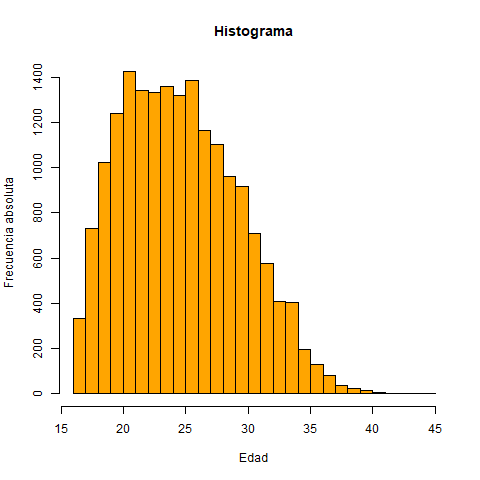
\includegraphics[width=\textwidth]{hist}


\bigskip
Procedemos a la separaci\'on de la variable en \textbf{clases de equivalencia} para calcular de ellas los distintos tipos de
frecuencia estudidados. Esto se hace gracias al uso de la librer\'ia \textbf{fdth} y para poder utilizarla, como se ha dicho 
anteriormente es necesario realizar lo siguiente:
\begin{Schunk}
\begin{Sinput}
> install.packages("fdth")
> library("fdth")
\end{Sinput}
\end{Schunk}

Procedemos al c\'alculo en s\'i:
\begin{Schunk}
\begin{Sinput}
> dist <- fdt(edad,breaks="Sturges")
> dist
\end{Sinput}
\begin{Soutput}
 Class limits    f   rf rf(%)    cf  cf(%)
      [16,18)  331 0.02  1.82   331   1.82
      [18,20) 1756 0.10  9.64  2087  11.46
      [20,21) 2663 0.15 14.63  4750  26.09
      [21,23) 2672 0.15 14.68  7422  40.76
      [23,25) 2677 0.15 14.70 10099  55.47
      [25,27) 1387 0.08  7.62 11486  63.09
      [27,29) 2263 0.12 12.43 13749  75.51
      [29,31) 1876 0.10 10.30 15625  85.82
      [31,32) 1281 0.07  7.04 16906  92.85
      [32,34)  812 0.04  4.46 17718  97.31
      [34,36)  323 0.02  1.77 18041  99.09
      [36,38)  119 0.01  0.65 18160  99.74
      [38,40)   25 0.00  0.14 18185  99.88
      [40,42)   18 0.00  0.10 18203  99.98
      [42,44)    1 0.00  0.01 18204  99.98
      [44,45)    3 0.00  0.02 18207 100.00
\end{Soutput}
\end{Schunk}

\begin{itemize}
\item Frecuencia absoluta -> f
\item Frecuencia relativa -> rf
\item Frecuencia relativa porcentual -> rf(\%)
\item Frecuencia abs acumulada -> cf
\item Frecuencia rel acumulada porcentual -> cf(\%)
\end{itemize}

\bigskip
Para calcular la \textbf{media} de edad hemos construido una funci\'on en R la cual es:
\begin{Schunk}
\begin{Sinput}
> source("media.R")
> media
\end{Sinput}
\begin{Soutput}
function(var) {
    sum<-0

    for (data in var) {
        sum<-sum+data
    }

    return(sum/length(var))
}
\end{Soutput}
\end{Schunk}

\bigskip
Procedemos al c\'alculo de la media haciendo uso de la misma:
\begin{Schunk}
\begin{Sinput}
> mf<-media(fifa$Age)
> mf
\end{Sinput}
\begin{Soutput}
[1] 25.12221
\end{Soutput}
\end{Schunk}

\bigskip
En cuanto a los \textbf{cuantiles}, para su visualizaci\'on hemos optado por el uso
de un diagrama de bigotes, donde adem\'as aparecen representados los l\'imites inferior
y superior de la variable de estudio. Para su realizaci\'on se ha hecho lo mismo que con el 
histograma de la siguiente manera:
\begin{Schunk}
\begin{Sinput}
> source("bigotes.R")
> bigotes
\end{Sinput}
\begin{Soutput}
function(var,ruta) {
    png(paste("./tmp/",ruta,sep=""))
 
    boxplot(var, col='green', horizontal=T) 

    dev.off()
}
\end{Soutput}
\end{Schunk}

\begin{Schunk}
\begin{Sinput}
> b<-bigotes(edad,"bigotes.png")
\end{Sinput}
\end{Schunk}
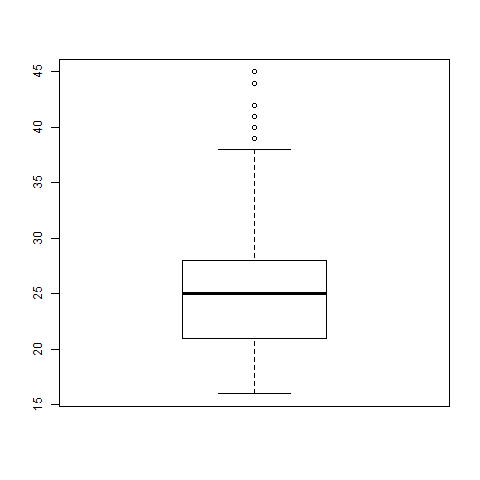
\includegraphics[width=\textwidth]{bigotes}

Para calcular la \textbf{desviaci\'on t\'ipica} hemos construido una funci\'on de la siguiente
forma:
\begin{Schunk}
\begin{Sinput}
> source("desviacion.R")
> desviacion
\end{Sinput}
\begin{Soutput}
function(var,media) {
    num<-0
    for (data in var){
        num<-num+((data-media)^2)
    }

    s<-sqrt(num/length(var))

    return(s)
}
\end{Soutput}
\end{Schunk}

El c\'alculo de la misma es:
\begin{Schunk}
\begin{Sinput}
> s<-desviacion(edad,mf)
> s
\end{Sinput}
\begin{Soutput}
[1] 4.669814
\end{Soutput}
\end{Schunk}

\bigskip
De acuerdo al teorema de \textit{Tchebychev} (realizado en una funci\'on aparte) el intervalo en el que se encuentran el 75\%
de los datos, es decir para k=2, es:
\begin{Schunk}
\begin{Sinput}
> source("tche.R")
> t<-tche(s,mf,2)
> toString(t)
\end{Sinput}
\begin{Soutput}
[1] "15, 34"
\end{Soutput}
\end{Schunk}

Dicha funci\'on es:
\begin{Schunk}
\begin{Sinput}
> tche
\end{Sinput}
\begin{Soutput}
function(des,media,k) {
    
    rango<-des*k
    inter<-list(as.integer(media-rango),as.integer(media+rango))

    return(inter)
}
\end{Soutput}
\end{Schunk}

Observando el intervalo tan amplio necesario para englobar el 75\% de los datos se puede concluir con que la media
no es una buena medida representante del conjunto de datos estudiado.

\bigskip
Por \'ultimo, el c\'alculo de la \textbf{varianza} es sencillo, \'unicamente es la desviaci\'on al cuadrado:
\begin{Schunk}
\begin{Sinput}
> v<-s^2
> v
\end{Sinput}
\begin{Soutput}
[1] 21.80717
\end{Soutput}
\end{Schunk}

\end{document}
